\chapter{相关工作}\label{chap:related_work}

\section{全美达公司的工作}

全美达公司在过去的几十年中在低功耗、兼容X86架构的微处理器领域取得了显著的成就。其代表性产品 Crusoe 系列微处理器于 2000 年首次推出,引起了业界的广泛关注。

全美达的工作重点是开发基于超长指令字(VLIW)处理器的微处理器,并结合软件侧的代码转换器,以实现低功耗、兼容X86的微处理器。

\subsection{代码转换器架构}

全美达的代码转换器\cite{dehnertTransmetaCodeMorphing2003}由解释器、运行时系统和动态二进制翻译器组成。在执行程序时,X86指令首先通过解释器进行解释执行并进行分析。根据代码块的执行频率,动态二进制翻译器逐步生成更优化的翻译,并将不同的指令组合成一条超长指令,指向底层硬件。这种方法类似于目前主流的多发射处理器的工作原理,在一拍内同时运行多条指令,通过动态地生成优化的超长指令来提高执行效率。

\subsection{Crusoe 微处理器}

全美达Crusoe 微处理器系列是该公司推出的兼容X86的微处理器,于 2000 年首次亮相。其中 Crusoe 以其实现 X86 兼容性的独特方式而著称。

Crusoe 运行的是一种称为代码转换器的软件抽象层或虚拟机,而不是在硬件中实现或由专用硬件进行转换的指令集架构。如图\ref{img:transmeta_arch}所示,代码转换器将从程序接收到的X86汇编代码指令翻译成微处理器的本机指令(超长指令字)。通过这种方式,Crusoe 也可以模拟其他指令集架构,例如Crusoe 也能将字节码翻译为其本机指令集中的指令来执行 Java 字节码。

这种架构的优势在于,通过在 X86 指令流和硬件之间引入抽象层,只需修改代码转换器,就可以在不破坏兼容性的情况下更改硬件架构。

\begin{figure}[h]
    \centering
    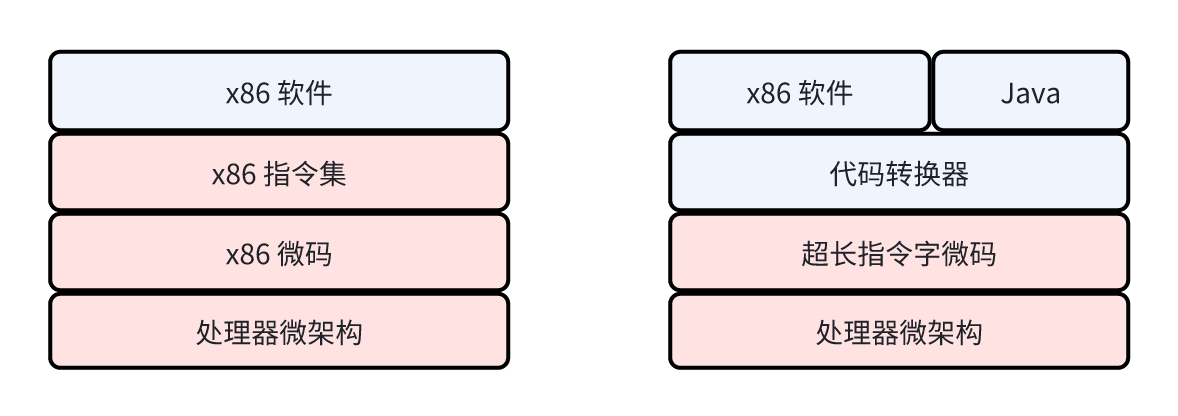
\includegraphics[width=0.8\linewidth]{./feishuImage/transmeta_arch.png}
    \caption{全美达架构图,在超长指令字处理器上实现兼容X86的指令集,并支持JAVA程序。}
    \label{img:transmeta_arch}
  \end{figure}


由于目前超标量乱序处理器的硬件乱序调度已经十分成熟,超长指令字设计在通用处理器上的流行度已经减弱,但全美达公司在多架构兼容性方面的工作提供了宝贵的经验,成为软硬结合二进制翻译器的重要先驱者。

\section{纯软件二进制翻译器的相关工作}

在纯软件领域,用户态二进制翻译器扮演着重要的角色。QEMU 是一款广泛使用的开源模拟器,支持多种指令集架构。如图\ref{img:qemu_arch},其核心目标之一是提供多架构的虚拟化支持,使用户能够在不同的硬件平台上运行其应用程序。它通过将不同指令集的机器代码翻译成中间语言(IR,Intermediate Representation),再将IR翻译成宿主指令集,实现跨架构的兼容性。这种设计使得QEMU能够处理多种指令集,为用户提供了一定的灵活性。然而,QEMU的性能仅能达到原生性能的13\%,这主要归因于双层翻译的性能损失。

\begin{figure}[h]
  \centering
  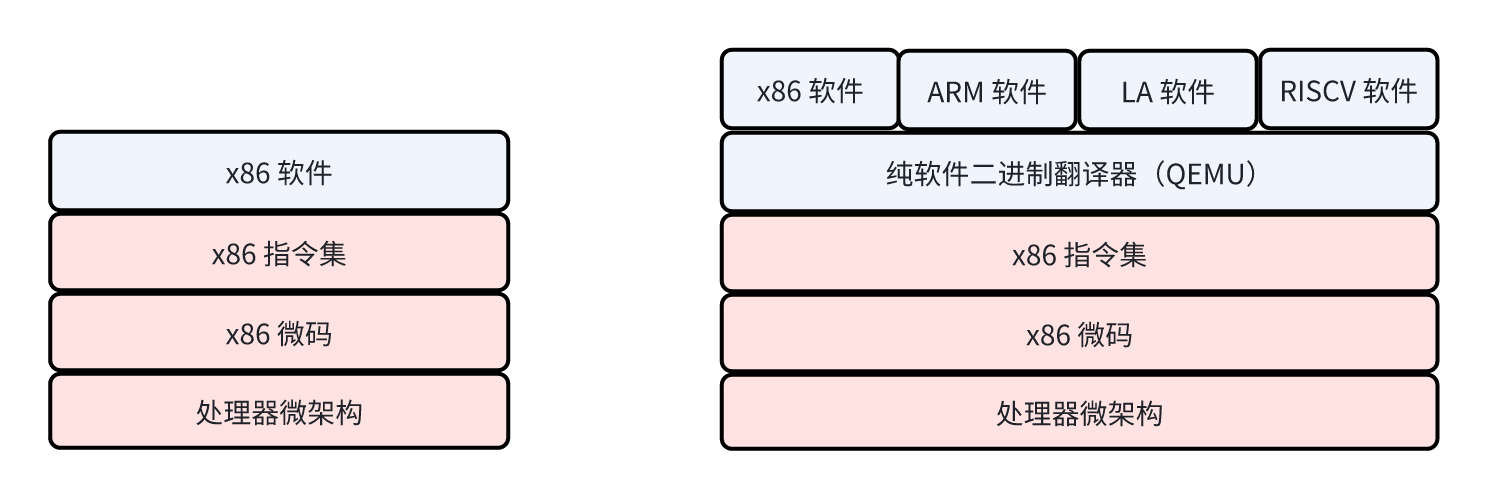
\includegraphics[width=0.8\linewidth]{./feishuImage/qemu_arch.png}
  \caption{QEMU二进制翻译器架构图,能在宿主指令集机器上运行多种客户程序。}
  \label{img:qemu_arch}
\end{figure}

尽管QEMU在实现多架构支持上取得了一些成功,但在性能方面仍然面临挑战。其性能仅相当于原生性能的一小部分,这在一些对性能要求较高的应用场景下显得不够可用。

其他常用的商用级用户级二进制翻译器,参见表\ref{tab:BTs},例如苹果公司的Rosetta2(67.2\%)、华为公司的ExaGear(72.7\%)、龙芯公司的LATX(60\%)等,性能上仍然无法接近原生性能。这些二进制翻译器采用一对一指令的翻译方式,即把一种指令集直接翻译到另一种指令集上(但一条客户指令可能翻译成多条宿主指令,产生指令膨胀,导致性能下降)。它们虽然在理论上支持多架构翻译,但实际上需要投入较大的工程量,也可能造成性能下降。

\begin{table}[]
\centering
\caption{主流二进制翻译器}
\label{tab:BTs}
  \begin{tabular}{llll}
  \rowcolor[HTML]{FBE5D6} 
  二进制翻译器    & 公司   & 客户平台           & 宿主平台           \\
  ExaGear   & 华为   & X86            & ARM            \\
  Rosetta2  & 苹果   & X86            & ARM            \\
  LoongArch & 龙芯   & X86            & LoongArch      \\
  QEMU      & 开源项目 & X86,ARM,RISCV等 & X86,ARM,RISCV等
  \end{tabular}
  \end{table}

\section{软件二进制翻译的性能开销来源}

\begin{figure}[h]
  \centering
  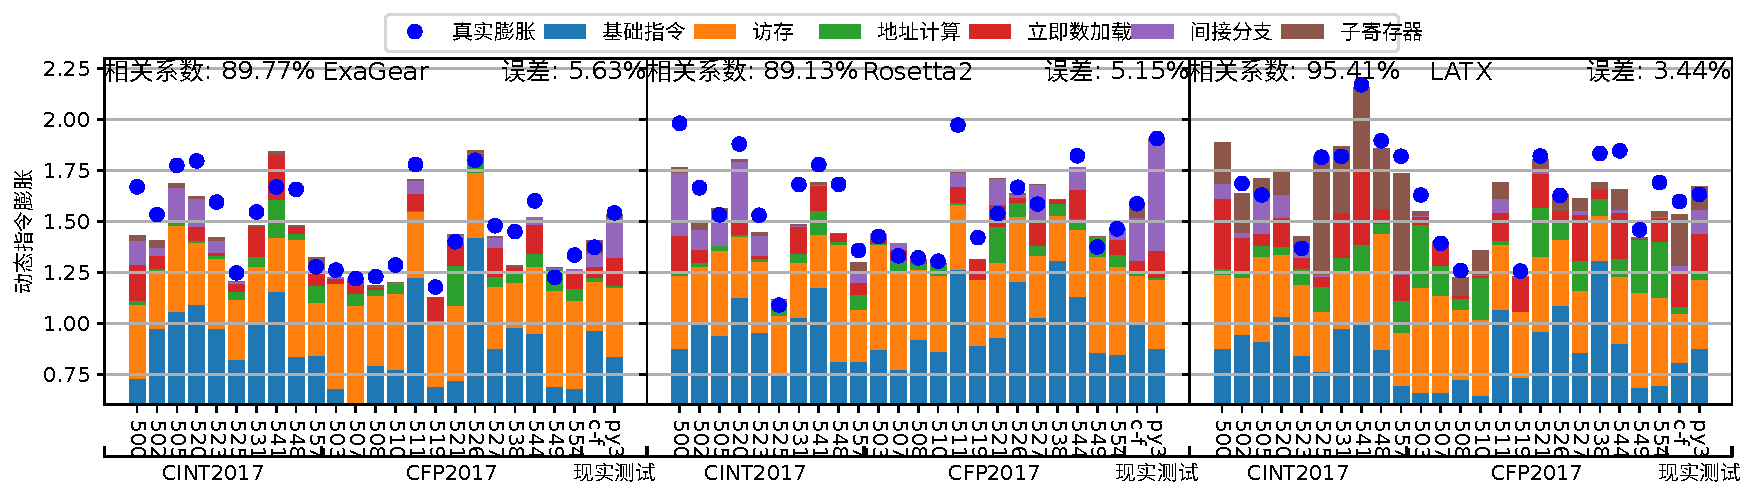
\includegraphics[width=1\linewidth]{./plot/insts_inflt_breakdown_2017.pdf}
  \caption{QEMU二进制翻译器架构图,能在宿主指令集机器上运行多种客户程序。}
  \label{img:insts_inflt_breakdown_2017}
\end{figure}

根据我们之前完成的一项工作,使用指令膨胀率来分析二进制翻译器的性能开销。指令膨胀率是指,每条客户指令平均翻译出的宿主指令数,是一个大于1的小数,计算方式为$\mbox{总体膨胀} = \mbox{生成的宿主指令数} / \mbox{客户指令数}$(这里用的是动态运行指令数)。指令膨胀率越高,翻译后的程序要执行的指令数越多,执行时间越长,性能越低。即便多发射处理器能在单拍内执行多条指令,缓解更多指令带来的性能开销,但根据我们的测试数据,指令膨胀率和性能下降值是保持正相关的。如图\ref{img:insts_inflt_breakdown_2017},我们主要把开销分成了5类:

%latex 使用1. 2. 3. 来编号
\begin{enumerate}
  \item \textbf{指令集间操作码差异:} 不同指令集的操作码差异引起Eflags计算等操作的额外指令翻译,增加了指令膨胀率。此外LoongArch对于子寄存器默认符号扩展,X86/ARM默认零扩展。对应图\ref{img:insts_inflt_breakdown_2017}中\textcolor{brown}{棕色}部分。
  
  \item \textbf{操作数据模式不同:} 复杂指令集(如X86)可以直接访问内存,而其他精简指令集只能操作寄存器,导致操作数模式不同。对应图\ref{img:insts_inflt_breakdown_2017}中\textcolor{orange}{橙色}部分。
  
  \item \textbf{地址计算不同:} 复杂地址计算方式(如X86)与其他指令集的简单计算方式导致在翻译时需要额外指令。例如X86计算地址$addr = base + index * scale +disp$; 其他的大多为$addr = base + offset$。 对应图\ref{img:insts_inflt_breakdown_2017}中\textcolor{green}{绿色}部分。
  
  \item \textbf{立即数加载:} X86支持编码64位立即数和32位地址偏移,而其他指令集编码空间有限,导致立即数加载的语义不同,需要额外的访存指令或者是多条立即数加载指令。对应图\ref{img:insts_inflt_breakdown_2017}中\textcolor{red}{红色}部分。
  
  \item \textbf{间接跳转:} 客户指令地址到宿主指令地址是非线性的,而间接跳转的目标地址在运行时才能知道,需要查询间接跳转哈希表,导致性能开销。对应图\ref{img:insts_inflt_breakdown_2017}中\textcolor{purple}{紫色}部分。
  
\end{enumerate}

以上这5类主要开销很难通过软件优化来解决,需要借助硬件辅助的方式来解决。

为了消除软件二进制翻译器的性能开销,特别是在处理指令集语义差异方面的挑战,本文采用了硬件辅助的策略。其中,一些关键的工作包括:

1. 融合微码以缩小指令集语义差距: 针对指令集间操作码差异、操作数据模式不同以及地址计算不同等问题,我们尝试通过融合微码的方式,减小不同指令集之间的语义差距,从而降低翻译的开销。

2. 微码缓存的思路应用: 针对立即数加载和间接跳转的性能开销,我们借鉴了X86微码缓存的思想,将立即数放入微码缓存行中直接加载,用微码缓存直接查询非线性的地址空间映射,消除这两类开销。

接下来,将介绍与X86微码缓存相关的工作,探讨如何借助硬件辅助手段进一步优化软件二进制翻译器的性能。


\section{X86 微码缓存的相关工作}

X86 微码缓存是为了在 X86 CPU 后端实现超标量乱序执行并降低译码功耗而引入的关键组件\cite{solomonMicrooperationCachePower2001},如图\ref{img:front_end_ucache}。以下是关于 X86 微码缓存的主要工作和设计特点:

\begin{figure}[h]
  \centering
  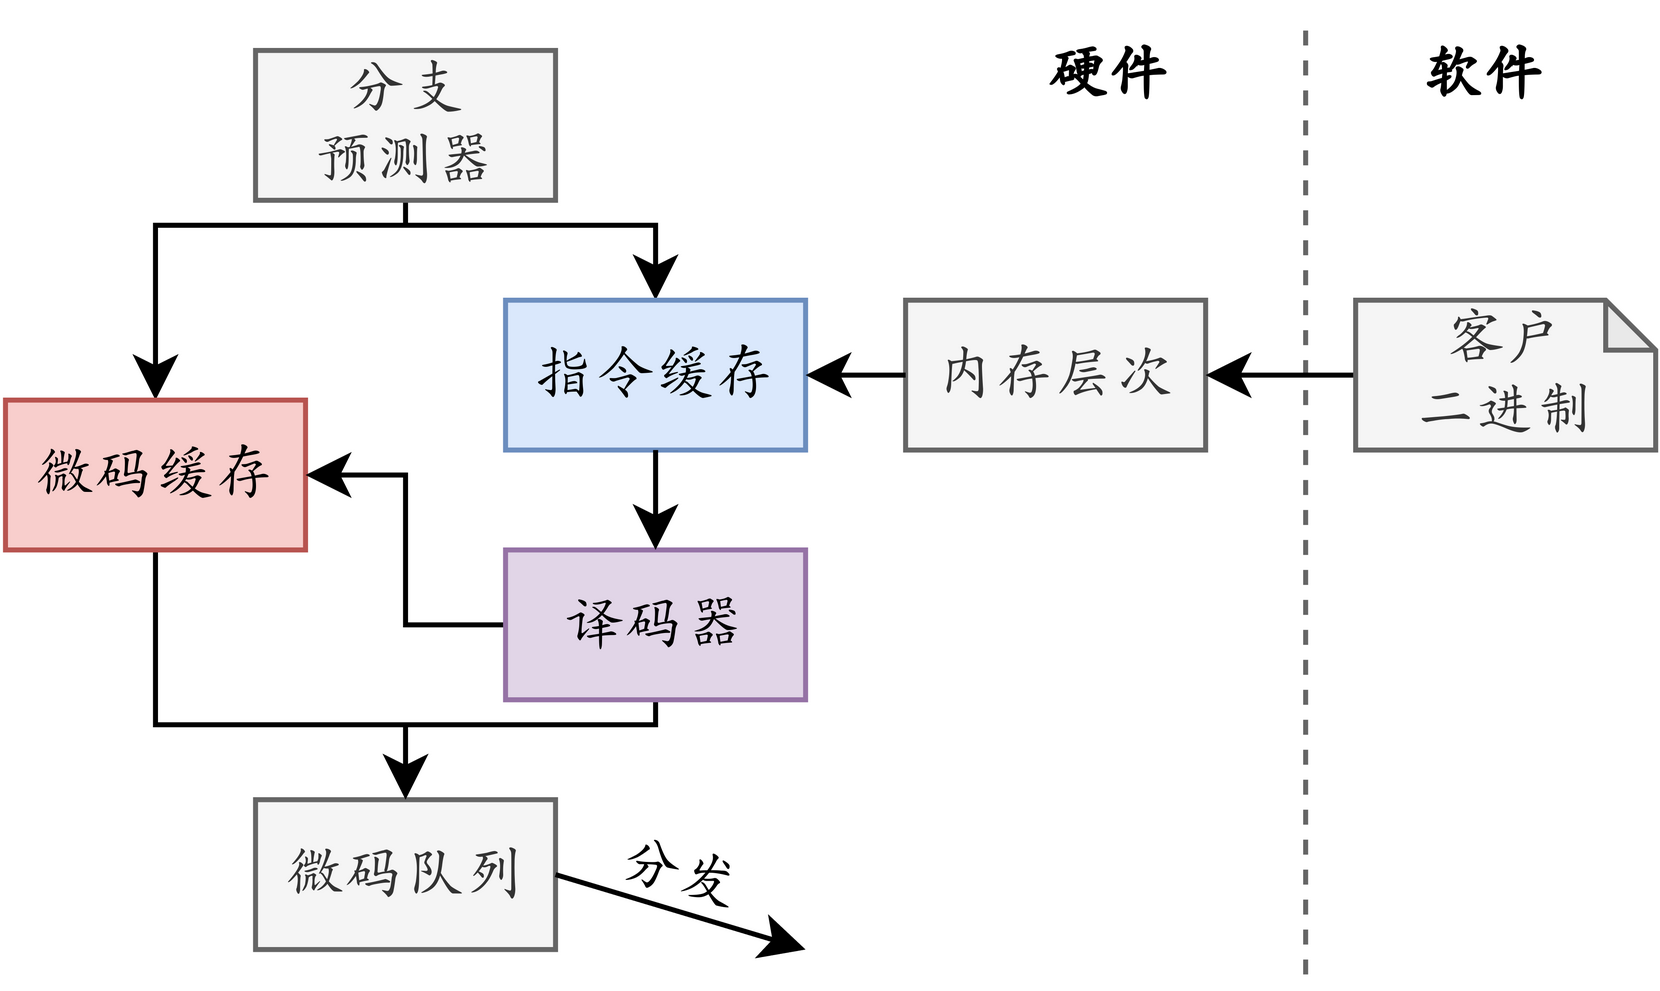
\includegraphics[width=0.8\linewidth]{./image/front_end_ucache.pdf}
  \caption{X86处理器前端架构图,包括指令缓存和微码缓存}
  \label{img:front_end_ucache}
\end{figure}

\begin{figure}[h]
  \centering
  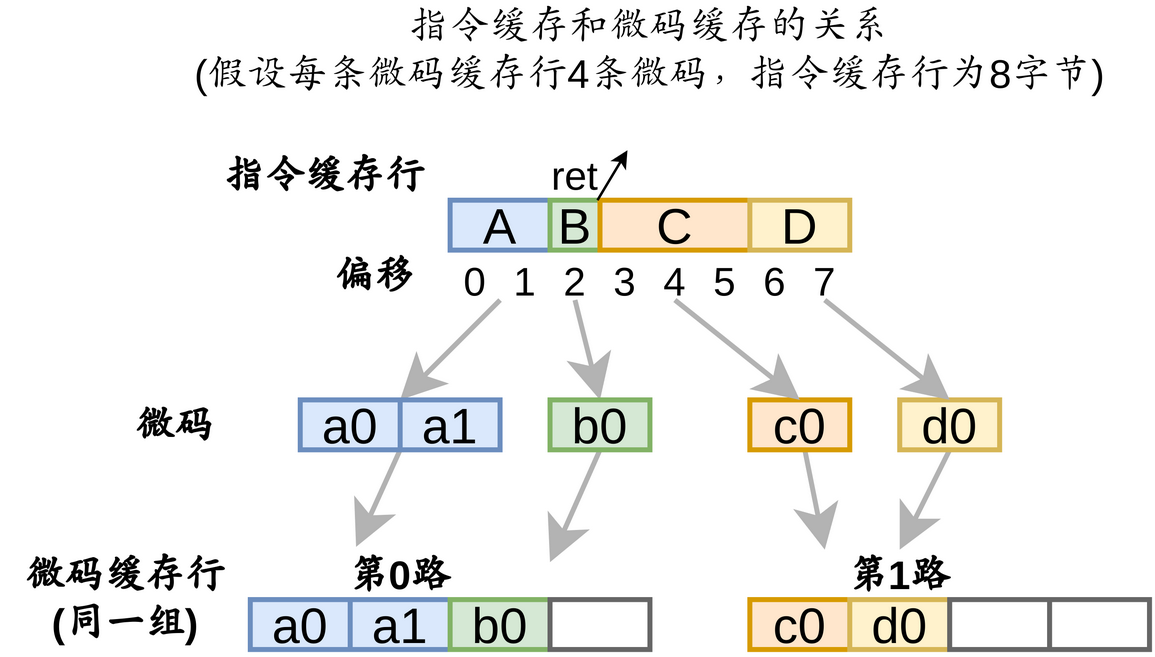
\includegraphics[width=0.8\linewidth]{./image/IC-to-UC.pdf}
  \caption{指令缓存和微码缓存关系}
  \label{img:IC_to_UC}
\end{figure}

1. \textbf{微码与超标量乱序执行的关系:}

   - 为了实现超标量乱序执行,X86 CPU 后端需要将复杂指令译码为简单指令,即微码。

   - 微码的引入简化了指令集的关系,使得 CPU 在后端能够更高效地执行。

2. \textbf{微码缓存的引入:}

- 为了降低译码能耗、提高性能,研究者们引入了微码缓存,用于存储已经译码过的微码。

- 微码缓存的设计目的是减少译码的重复计算,从而提高整体指令执行效率。

3. \textbf{查询与缓存机制:}
  
- 在前端译码阶段,系统首先查询微码缓存,检查是否已经缓存了当前指令的微码。

- 如果微码已经在缓存中,CPU 就直接读取微码并发射到后端执行。

- 如果微码未缓存,系统则从指令缓存中取得指令,进行译码,并将译码结果存入微码缓存中,见图\ref{img:IC_to_UC},注意一个指令缓存行可能生成多个微码缓存行。

4. \textbf{缓存组织形式:}

- 微码缓存的组织形式与指令缓存有所区别。它以第一条指令的程序计数器(PC)作为索引,来索引整行的微码。

- 当遇到控制流指令时,微码缓存会截断这一行,确保每个缓存行只包含一个基本块的微码,参考图\ref{img:IC_to_UC}中的ret指令。

- 微码行中除了存入微码外,还会在最后存储立即数,见图\ref{img:ucache_line},这是由于X86是变长指令集,微码是定长指令集,遇到长立即数时候就会放在微码行最后。

X86 微码缓存的引入和优化为 X86 架构的超标量乱序执行提供了重要支持,使得 CPU 在执行 X86 指令集时能够更加高效地利用硬件资源,提高整体性能。

\begin{figure}[h]
  \centering
  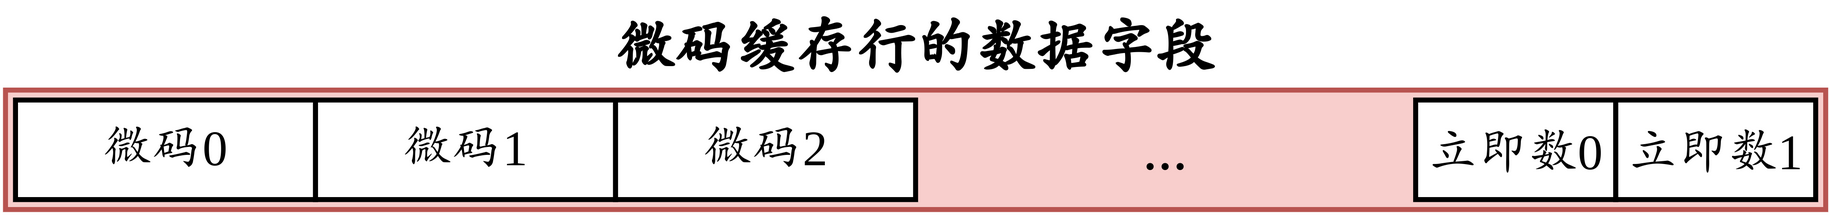
\includegraphics[width=0.8\linewidth]{./image/ucache_line.pdf}
  \caption{指令缓存和微码缓存关系}
  \label{img:ucache_line}
\end{figure}
